\documentclass[Kravspecifikation/Kravspec_Main.tex]{subfiles}
\begin{document}
\section{Ikke-funktionelle krav}
De ikke funktionelle krav beskriver systemets fysiske dimensioner, fysiske parameter, og det forskellige GUI. Herudover beskriver det også en række specifikationer om systemet ydeevne. For specifik forklaring, se Definitionsliste (side xx).

Til at beskrive nogle af kravene er der nogle skitser som hjælper med at forklare kravene. 

\subsection{Fysiske Parametre}
Dimensioner bliver angivet i følgende format [længde/bredde/højde][cm]
\begin{table}[H]
\centering
\begin{tabular}{|L{0.1\textwidth}|L{0.6\textwidth}|L{0.15\textwidth}|}
\hline
\textbf{ID} & \textbf{Krav} & \textbf{Prioritet} \\ \hline
K1.1 & Beer Pong bordet skal være 240cm/60cm/70cm +/- 1cm  &  \\ \hline
K1.2 & Systemet skal kunne håndtere en Ball med en diameter på 40mm +/- 1mm&  \\ \hline
K1.3 & Display'ets billede skal være 24 tommer +/- 0.5 tommer diagonalt med et format på 16:9&  \\ \hline
K1.4 & Systemet skal kunne håndtere kopper med en øvre diameter på $94\si{mm} \pm 3\si{mm}$ og en nedre diameter på $65\si{mm} \pm 3\si{mm}$  og en højde på $120mm \pm{5mm}$ & \\ \hline
K1.5 & Systemet skal kun tage imod en dansk femkrone som betaling. Diameter på 28.5 mm +/- 0.5mm og tykkelse på 2.00 +/- 0.1 mm & \\ \hline
K1.6 & Systemet skal returnere mønter med en diameter på 27.0 mm og under og tykkelse på 2.35 mm og under & \\ \hline
K1.7 & Systemet skal ikke tage imod returnere mønter med en diameter på 29.0 mm og over og tykkelse på over 2.35 mm& \\ \hline
K1.8 & $D_{inner}$ på figur \ref{fig:LEDplacement} skal være $55\si{mm} \pm 1\si{mm}$  & \\ \hline
K1.9 & $D_{center}$ på figur \ref{fig:LEDplacement} skal være $65\si{mm} \pm 1\si{mm}$  & \\ \hline
K1.10 & $D_{led}$ på figur \ref{fig:LEDplacement} skal være $5\si{mm} \pm 1\si{mm}$  & \\ \hline
K1.11 & $D_{outer}$ på figur \ref{fig:LEDplacement} skal være $75\si{mm} \pm 1\si{mm}$   & \\ \hline
K1.12 & Vinklen mellem to LED'er i CupLight skal være $70^{\circ} \pm 2^{\circ}$ & \\ \hline
K1.13 & Afstanden mellem to CupHolders skal være $100\si{mm} \pm 2\si{mm}]$ & \\ \hline
K1.14 & Systemet skal fungere med $110\si{ml} \pm 20\si{ml}$ Ceres Top øl i hver Cup & \\ \hline
K1.15 & Systemet skal fungere med en almindelig hvid bordtennis bold & \\ \hline
K1.16 & Systemet skal detektere en bold der falder fra en højde på 30cm over bordet. & \\ \hline 
K1.17 & Systemet skal detektere placering af en Cup når centrum af Cup og centrum af CupHolder er under 10mm & \\ \hline

\end{tabular}
\caption{Ikke funktionelle krav for de fysiske dimensioner}
\label{tab:fysiske_dimensioner}
\end{table}


\subsection{User Interface}
Der er lavet en skitse der beskriver hvordan en Cup holder ser ud. Dette kan ses på figur \ref{fig:LEDplacement}

\begin{figure}[H]
    \centering
    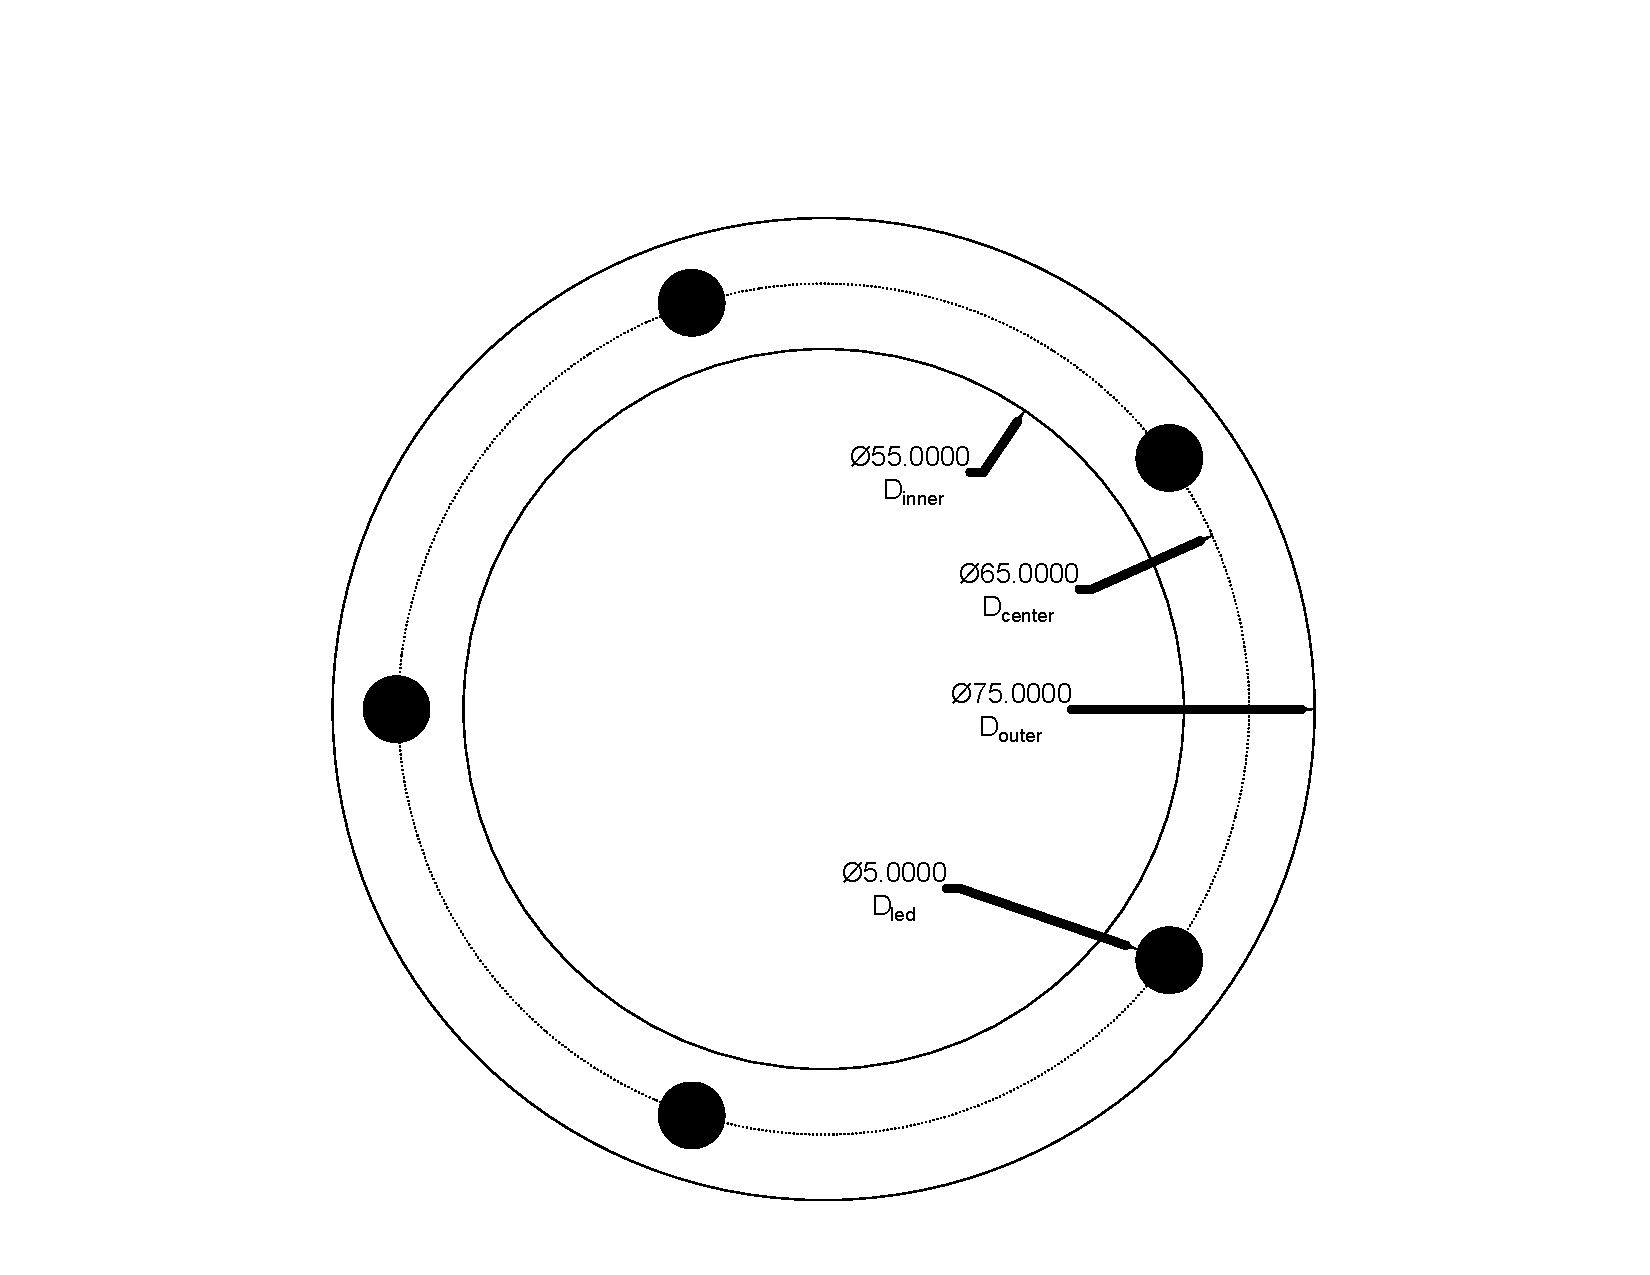
\includegraphics[width=0.8\textwidth,trim={2in 0.4in 2in 1.3in},clip, page=1]{Kravspecifikation/Ikke-funktionelle/graphics/LEDplacement.pdf}
    \caption{Skitse der viser de forskellige dele af en cup holder. Der er påtegnet forskellige diametre med mål. Målenes tolerance er specificeret i tabel \ref{tab:fysiske_dimensioner}.}
    \label{fig:LEDplacement}
\end{figure}

På figur \ref{fig:LEDplacement} er der en ring af lys (Cup light). Denne ring er afgrænset af den indre cirkel (med diameteren $D_{inner}$ og den ydre cirkel (med diameteren $D_{outer}$). De 5 sorte cirkler (med diameteren $D_{led}$) repræsenterer LED'er som er lyskilderne i Cup light. De er placeret på en cirkel med diameteren $D_{center}$. LED'ernes placering $(D_{led})$ er valgt ud fra at passe med de fysiske krav på en kop (se krav i ).
\begin{table}[H]
\centering
\begin{tabular}{|L{0.1\textwidth}|L{0.65\textwidth}|L{0.15\textwidth}|}
\hline
\textbf{ID} & \textbf{Krav} & \textbf{Prioritet} \\ \hline
K2.1 & Systemet skal hoste et wifi netværk med SSID ''Beer\_Pong\_Table'' og adgangskoden ''beerpong''. & \\ \hline
K2.2 & Når alt er sat op (der er glas på bordet og betalt for bolde) må der som maksimum kun gå 10 sekunder før spillets &  \\ \hline
%K2.3 & Displayskærmen på bordet skal kunne vise et spillers navn og score hurtigere end 5 sekunder efter, at man har tastet sit navn på mobilappen og trykket ok. &  \\ \hline
K2.3 & Displayskærmen skal kunne vise \textit{\textbf{spil status}} og \textit{\textbf{spiller oplysninger}} samtidigt. & \\ \hline
K2.4 & De fem LED'er i CupLight til en CupHolder skal lyse med den samme farve. & \\ \hline
K2.5 & Et enkelt CupLight skal kunne lyse med mindst 10 forskellige farver & \\ \hline
K2.5 & Hvert CupLight skal kunne styres individuelt & \\ \hline 
K2.6 & Et CupLight skal i UC1 lyse gul når der ikke er en Cup i den tilhørende Cup holder  & \\ \hline
K2.7 & Et CupLight skal i UC1 lyse blå når der ikke er en Cup i den tilhørende Cup holder & \\ \hline
K2.8 & StatusLED skal bestå af to lysdioder &  \\ \hline
K2.9 & Lysdioderne på StatusLEDlyser i to forskellige farver, rød og grøn &  \\ \hline
K2.10 & Den røde lysdiode i StatusLED lyser, når der er mindre end to bolde tilbage i BallDispenser &  \\ \hline
K2.11 & Den grønne lysdiode i StatusLED skal tændes, når BallDispenser er fuld af bolde &  \\ \hline
\end{tabular}
\caption{Ikke funktionelle krav for User Interface}
\label{tab:user_interface}
\end{table}

\subsection{Ydeevne}
\begin{table}[H]
\centering
\begin{tabular}{|L{0.1\textwidth}|L{0.65\textwidth}|L{0.15\textwidth}|}
\hline
\textbf{ID} & \textbf{Krav} & \textbf{Prioritet} \\ \hline
K3.1 & Bolddispenser skal levere den første af to bolde indenfor 5s efter der indsættes en mønt. &  \\ \hline
K3.2 & Når en spiller/hold har vundet (\textit{\textbf{Spillet er slut}}), skal systemet vise hvem der har vundet indenfor 100 ms. &  \\ \hline
K3.3 & Systemet skal være vandtæt. Dvs. øl, sodavand og andet væske ikke kan kom til systemet indre sensorer eller computer, uden at bordets top fjernes. &  \\ \hline
K3.4 & Systemets \textbf{\textit{start op}} og \textbf{\textit{slukke}} tid skal være mindre end 10 sekunder. &  \\ \hline
K3.5 & Display'et skal vise at en person har fjernet et kop fra en kopholder indenfor 500ms. &  \\ \hline
K3.6 & Bolddispenseren skal kunne indeholde 14 bolde. & \\ \hline
\end{tabular}
\caption{Ikke funktionelle krav for ydeevne}
\label{tab:ydeevne}
\end{table}

\subsection{Pålidelighed}
\begin{table}[H]
\centering
\begin{tabular}{|L{0.1\textwidth}|L{0.65\textwidth}|L{0.15\textwidth}|}
\hline
\textbf{ID} & \textbf{Krav} & \textbf{Prioritet} \\ \hline
K4.1 & Det skal med et konfidensniveau på 95\% detekteres at der placeres en \textbf{Cup} i en kopholder.  &  \\ \hline
K4.2 & Det skal med et konfidensniveau på 95\% detekteres at der løftes en \textbf{Cup} fra en kopholder.  &  \\ \hline
K4.3 & Det skal med et konfidensniveau på 95\% detekteres at en \textbf{Ball} rammer i  en \textbf{Cup} som står i en kopholder. Bolden skal tabes med en højde på 30cm over bordoverfladen &  \\ \hline
K4.4 & I en periode på 1 time uden ydre påvirkninger af systemet må der højest være 1 falsk detektering af placering af en \textbf{Cup} på tom kopholder &  \\ \hline
K4.5 & I en periode på 1 time uden ydre påvirkninger af systemet må der højest være 1 falsk detektering af løfting af en \textbf{Cup} fra kopholder hvor der står en kop&  \\ \hline
K4.6 & Når en \textbf{Ball} rammer en kopholder og hopper væk igen 100 gange (uden nogen \textbf{Cup}) må der højest ske 1 falsk detektering af at der placeres en \textbf{Cup} i den givne kopholder&  \\ \hline
K4.7 & Det skal detekteres mindst 98 ud af 100 gange at der indsættes en 5 krone i bolddispenser. &  \\ \hline
K4.8 & Det skal detekteres højst 2 ud af 100 gange at der indsættes en 5 krone i bolddispenser når der indsættes enhver anden dansk mønt. &  \\ \hline
K4.9 & I en periode på 1 time uden ydre påvirkninger af systemet må der højest være 1 falsk detektering af indsættelse af en dansk 5 krone i bolddispenser &  \\ \hline
K4.10 & Der må højst ske en fejl ved levering af 2 \textbf{Balls} (dvs. der leveres mindre eller flere end 2 \textbf{Balls}), 1 ud af 50 gange der sendes signal om at der skal leveres 2 \textbf{Balls}.  &  \\ \hline


\end{tabular}
\caption{Ikke funktionelle krav for pålidelighed}
\label{tab:reliability}
\end{table}

\subsection{WebPage}
\begin{figure}[H]
    \centering
    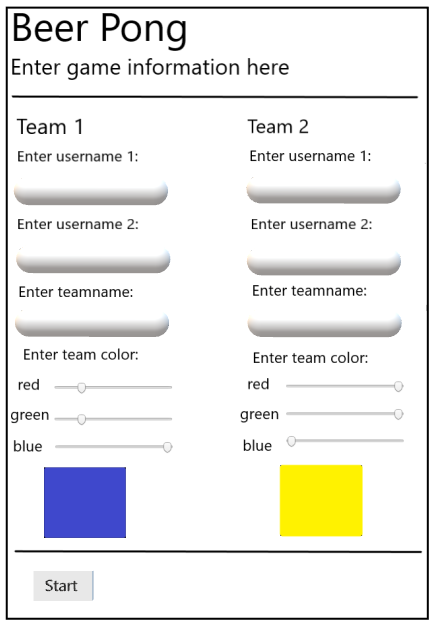
\includegraphics[width=0.6\textwidth]{Kravspecifikation/Ikke-funktionelle/graphics/WebPage_IF.png}
    \caption{Skitse af grænsefladen for WebPage}
   \label{fig:WebPage_IF}
\end{figure}

\begin{table}[H]
\centering
\begin{tabular}{|L{0.1\textwidth}|L{0.65\textwidth}|L{0.15\textwidth}|}
\hline
\textbf{ID} & \textbf{Krav} & \textbf{Prioritet} \\ \hline
K5.1 & WebPage er en hjemmeside med statisk IP-adresse 10.9.8.2, som hostes af en RPi. & \\ \hline
K5.2 & Alt tekst på hjemmesiden er på sproget engelsk. & \\ \hline
K5.3 & RPi er konfigureret som hotspot, så hjemmesiden kan tilgås via smartphone. & \\ \hline
K5.4 & På hjemmesiden skal der for hvert af de to hold indtastes følgende oplysninger: \textit{teamname}, \textit{username1} og \textit{username2}. & \\ \hline
K5.5 & Holdnavne og brugernavne indtastet på hjemmesiden skal være tekststrenge, med en længde på mellem 1 og 15 karakterer. & \\ \hline
K5.6 & På hjemmesiden skal der for hvert af de to hold kunne vælges holdfarve ved at justere intensiteten af farverne rød, grøn og blå i et RGB farveskema. & \\ \hline
K5.7 & Hver af farverne rød, grøn og blå tildeles en integer værdi mellem 0 og 255, hvor 0 er lavest og 255 er højest. Der skal dermed kunne vælges imellem 256*256*256=16.777.216 farver.  & \\ \hline
K5.8 & Når oplysningerne sendes, må der højst gå 0,1 sekund, før der modtages et svar fra serveren. & \\ \hline
K5.9 & Der må højst ske en fejl i afsendingen 1 ud af 50 gange. & \\ \hline
\end{tabular}
\caption{Ikke funktionelle krav for WebPage}
\label{tab:WebPage}
\end{table}

\subsection{LEDs}

\subsection{GUI}
\begin{table}[H]
\centering
\begin{tabular}{|L{0.1\textwidth}|L{0.65\textwidth}|L{0.15\textwidth}|}
\hline
\textbf{ID} & \textbf{Krav} & \textbf{Prioritet} \\ \hline
K8.1 & GUI systemet skal kunne skfite fra et baggrunds billede til et nyt, på under et sekund: efter der modtages et signal fra RPI'en.  & \\ \hline
K8.2 & GUI systemet skal kunne skifte kop farven for en given kop på under 1 sekund +-0.5 sekunder, efter der modtages et signal fra RPI'en. & \\ \hline
K8.3 & GUI systemet skal ikke håndtere nogen form for logisk "spiller oplysninger" eller "spil status", men kun vise hvad RPI'en sender & \\ \hline
K8.4 & PAlt funktionellitet fra GUI systemet skal kun styres fra RPI'en & \\ \hline
K8.5 & Efter "start op" processen påbegynder må der maks gå 10 sekunder til at gui'en skal være funktionsdygtig. & \\ \hline
K8.6 & Gui'en skal være funktionsdygtig mindst 95\% +- 1\% tiden systemet er i brug. & \\ \hline
K8.7 & Hvad Displayet viser skal være nøjagtig til hvad den rigtige "spil status" er 99\%  af tiden, +- 1\%. & \\ \hline
\end{tabular}
\caption{Ikke funktionelle krav for GUI}
\label{tab:GUI}
\end{table}

\end{document}